
\documentclass{article}
%\documentclass[preprint, prb]{revtex4-1}
\usepackage{amsmath,amssymb,amsfonts,mathrsfs,slashed,amstext,array,blkarray,amsthm,amssymb}
\usepackage{graphicx}
\usepackage{svg}
%\usepackage{multicol} % only for \documentclass{article}
%\usepackage{mathabx} % only for \documentclass{article}
%\usepackage{mathtools, cuted}  % only for \documentclass{article}
%\usepackage{svg} % only for \documentclass{article}
\usepackage{enumitem}
\usepackage[toc,page]{appendix}
\usepackage{bm,bbold}
\usepackage[font={footnotesize}]{caption}
\usepackage{todonotes}
\usepackage{comment}
\usepackage{changepage}
%\usepackage{epsfig,subcaption,float,graphicx}
\usepackage{multirow}
\usepackage{multicol}
\usepackage{verbatim}
\usepackage{tkz-euclide}

\graphicspath{{./}{./Figs/}}
\definecolor{darkblue}{rgb}{0.1,0.2,0.6} \definecolor{darkred}{rgb}{0.8,0.1,0.2}
\usepackage[colorlinks,citecolor=darkblue,linkcolor=darkred,urlcolor=darkblue]{hyperref}
\usepackage[all]{hypcap}


\renewcommand{\vec}[1]{\boldsymbol{\mathbf{#1}}}

\newcommand{\cf}{\textit{cf.} } 
\newcommand{\ie}{\textit{i.e.} } 
\newcommand{\eg}{\textit{e.g.} }
\newcommand{\vs}{\textit{vs.} } 
\newcommand{\etal}{\textit{et al.} }
\newcommand{\etc}{\textit{etc.} }
\newcolumntype{L}{>{$}l<{$}} % math-mode version of "l" column type

\textwidth = 6.5 in
\textheight = 9 in
\oddsidemargin = 0.0 in
\evensidemargin = 0.0 in
\topmargin = 0.0 in
\headheight = 0.0 in
\headsep = 0.0 in
\parskip = 0.2in
\parindent = 0.0in
% document begins

\begin{document}
%\maketitle
\begin{figure}
\centering
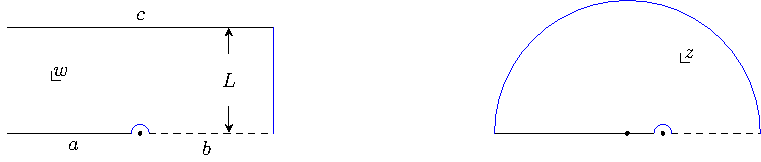
\includegraphics[width=\columnwidth]{/images/fig_fidel-map.pdf}
\caption{?}
\label{fig:Conformal_transformation}
\end{figure}

We would like to consider the following conformal transformation in Fig.~\ref{fig:Conformal_transformation}. We first map the stripe on the $\omega$-plane to a semicirlce on the $z$-plane, and then map it to two concentric circles on $z'$-plane, and finally maps it to a cylinder on the $\xi$-plane. 

The UV regulator on the $z$-plane was spanned across $\exp\pm\pi\frac{\epsilon}{L}$ while the IR regulator was spanned across $\pm \exp\pi\frac{W}{L}$ where $W$ is the IR regulator on the $\omega$-plane. 

We want to map it to two concentric circles on $z'$-plane, to the first order of $\epsilon$. First we want to illustrate that the following map
\begin{eqnarray}\begin{aligned}
z'(z)&=\frac{z-a}{az-1}
\end{aligned}\end{eqnarray}
does not work. First $z'(1)=-1$, thus $a$ and $b$, which roughly are $a\pm\epsilon$ should be around $-1$ rather than around the origin. Indeed, we can simply expand
\begin{eqnarray}\begin{aligned}
\frac{1\pm\epsilon-a}{a(1\pm\epsilon)-1} = \frac{1-a\pm\epsilon}{a-1}\left(1\mp\frac{a}{a-1}\epsilon\right) = -1\pm\frac{1+a}{a-1}\epsilon
\end{aligned}\end{eqnarray}
as it should be.

The map we may want is 
\begin{eqnarray}\begin{aligned}
z'(z) = \frac{1}{z-1}
\end{aligned}\end{eqnarray}
which intuitively makes sense. Let's check
\begin{eqnarray}\begin{aligned}
z'(\exp\pm\pi\frac{\epsilon}{L}) &= \pm\frac{L}{\pi\epsilon} \\
z'(\pm\exp\pi\frac{W}{L}) &= \pm\exp\pi\frac{-W}{L} \\
\end{aligned}\end{eqnarray}
Thus the IR and UV regulator exchange places in the $z'$-plane, and they are concentric. We note also that the relative position of the solid and dash line does not change. 

And finally the map from $z'$ to $\xi$ would be $\xi = \ln z'$ such that it is mapped from circle to stripe. Thus The complete map is 
\begin{eqnarray}\begin{aligned}
\xi(\omega) = \ln\frac{1}{\exp\frac{\pi\omega}{L}-1}
\end{aligned}\end{eqnarray}
Let's check. The boundary condition of a is $(-\infty,-\epsilon)$ and $b$ is $(\epsilon,W)$ and $c$ is $(-\infty+iL,W+iL)$, they are mapped to
\begin{eqnarray}\begin{aligned}
a&: (-i\pi,-\ln\frac{\pi\epsilon}{L}-i\pi) \\
b&: (-\ln\frac{\pi\epsilon}{L},-\frac{\pi W}{L}) \\
c&: (-i\pi,-\frac{\pi W}{L}-i\pi) \\
\end{aligned}\end{eqnarray}
which is a cylinder with width $\pi$ and length $-\ln\frac{\pi\epsilon}{L}+\frac{\pi W}{L}$. The length go to infinity with $\epsilon\rightarrow0$ and $W\rightarrow\infty$. 

It is clear from the map $\xi(\omega)$ that the minus sign in front of the log-function is irrelevant, namely the map $z'(z)$ can really be taken as $z'(z)=z-1$ rather than $z'(z)=\frac{1}{z-1}$, as we did here. 

%\end{comment}

\end{document}